\chapter{Pushing I: Making NAF sweat}
\label{sec:push_sim_1}

Previous experiments showed that using NAF, a policy can be learned both in
simulation and on real robots to perform a reaching task to arbitrarily set
goal positions within the workspace. Extending this, we want to investigate
whether an object can be pushed to these goal positions. Preliminary
experiments on the real robotic systems on a cube pushing task using NAF did
however not converge to an intuitively good policy. To further investigate the
capabilities of the NAF algorithm under more controlled circumstances,
simulation experiments were first done.

\section{Method}

\subsection{Definition of the MDP}

The set of states
\begin{equation}
    S \subset \mathbb{R}^2 \times \mathbb{R}^2 \times \mathbb{R}^2
\end{equation}
was extended by including the center position of a pushable, circular, object.
The set of actions was defined in the same way as previous experiments. The
state transitions are now not as straightforward to describe as in the
simulated reaching task since they depend on a physics model, albeit a simple
one, for moving the object after contact with the simulated end-effector. The
object was modeled to have no velocity, and since this is the case, a state
only including positions still satisfies the Markov property.

The reward was defined from the state of the end-effector $\mathbf{e}$ and the
object $\mathbf{c}$, both in the successor state. The goal $\mathbf{g}$ was constant
before and after actions:
\begin{equation}
    r(\mathbf{e, c, g}) = \exp ( -k_1 ||\mathbf{e - c}||) + \exp (-k_2 ||\mathbf{c - g}|| )
\end{equation}
During the experiments, several values were tried for $k_1$ and $k_2$.

\subsection{Environment}

The environment consisted of the circular object to push into some goal
position, and a simulated, point-like end-effector. To simplify the problem,
locations of the pushable object and goal were sampled approximately at the
same position at every reset. This was in order to ignore rotations and
translations of the problem and only examine whether the algorithm could learn
this simpler scenario. The simulated end-effector was sampled uniformly in the
entire workspace. There was at this stage a concern that when the end-effector
has to go 180 degrees around the object, a clear multi-modal solution exists
and might be problematic due to the quadratic shape of the advantage function.
To further make this point clear, moving the end-effector clockwise around the
pushable object, or counter-clockwise, are equally good.  But staying at the
same position, or even worse moving towards the object pushing the object
further from the goal, lowers the return. Clearly, this has a multi-modal
nature, with one mode being going around the object clockwise, and the other
going counter-clockwise. 

\subsection{Algorithms}

The NAF algorithm was used where the network consisted of 2 hidden layers of
200 ReLU activated units each. The activation function for the $\mu$ output was
a tanh-function scaled by $0.01$, the environment was also changed to cap
actions with norm larger than this distance. A prioritized experience replay
buffer was used to store and sample mini batches of size $64$. Samples were
drawn with probability proportional to $p_i = |\delta_i| + \epsilon$, where
$\delta_i$ is the latest temporal difference error of sample $i$ and $\epsilon
= 10^{-9}$.  The loss for each sample $i$ was scaled by using importance
sampling weights $\left( \frac{1}{p_i}\right) ^\beta$ where $\beta$ was
linearly annealed from $0$ to $1$. A decay factor $\gamma = 0.99$ was used.

\section{Results}

The algorithm was able to approach the pushable object, but unable to push it
to the target position including going around the object to push it towards the
target. This is illustrated in figure \ref{fig:naf_sim_failure}. In figure
\ref{fig:naf_sim_unimode_q}, the Q-function is shown for a scenario where
intuitively the optimal policy should be to go up or down, but not left or
right. It is unclear if this is due to the quadratic shape of the advantage
function being unable to represent this, or some other detail in the
implementation. By an intuitive policy, what is meant is to never push the
object until the end-effector is positioned on the correct side of the object,
but naturally another possible policy could be to push the object in a circle
towards the goal. This did however not happen when evaluating the policy by
running test runs in the environment, as can be seen in figure
\ref{fig:naf_sim_failure}.

\begin{figure}[h!]
    \centering
    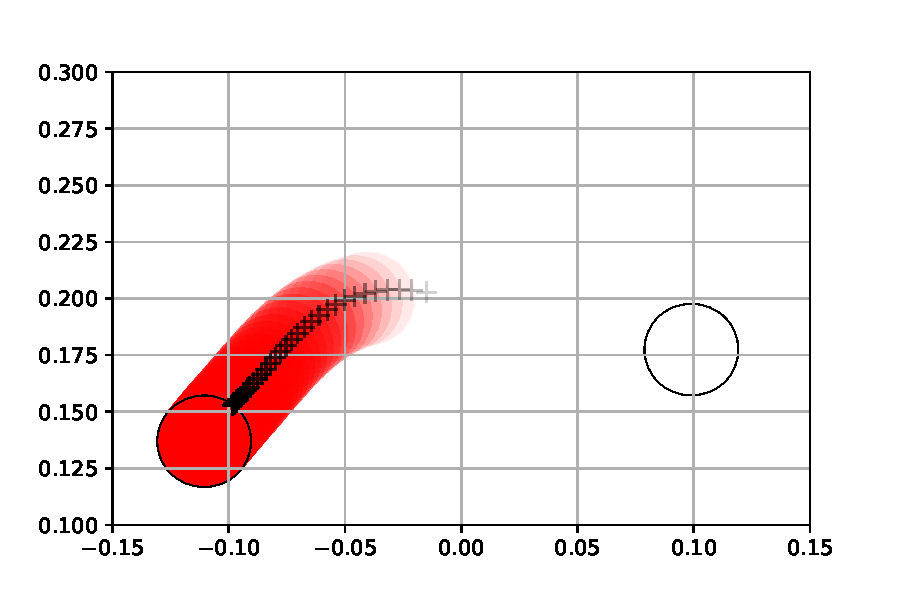
\includegraphics[width=0.4 \textwidth]{res/naf_sim_failure_mode.pdf}
    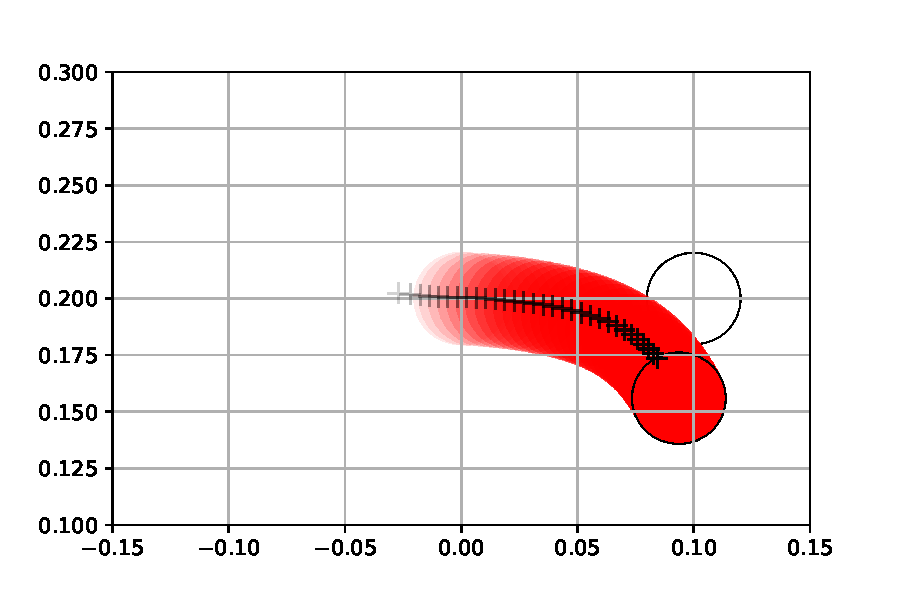
\includegraphics[width=0.4 \textwidth]{res/naf_sim_failure_mode_ideal.pdf}

    \caption{Results of NAF in simulation on pushing task. The red circle is
    the object being pushed, the white circle is the goal, and the cross is the
    simulated end-effector.}

    \label{fig:naf_sim_failure}
\end{figure}

\begin{figure}[h!]
    \centering
    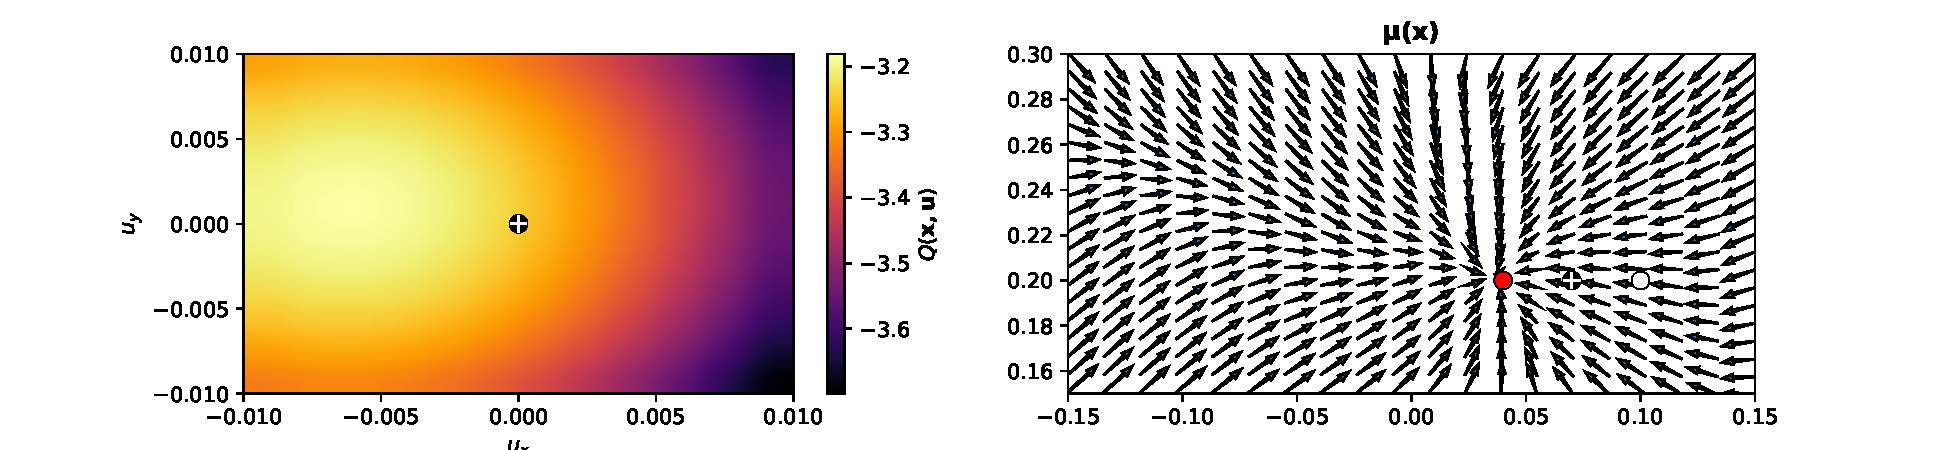
\includegraphics[width=1.0 \textwidth]{res/naf_sim_unimode_q.pdf}

    \caption{Results from using NAF on a simulated pushing task. Q-function and
    policy of the state given by the pushable object (red), the goal (white
    circle), and the end-effector (white cross). Since the advantage function
    is parameterized by a quadratic expression, which is uni-modal, the
    Q-function cannot represent the bi-modal nature of this scenario.}

    \label{fig:naf_sim_unimode_q}
\end{figure}
